% !TeX root = ../tesis.tex


\chapter{Ajuste con el modelo de Lorentz}

\label{section:apendix1}

En la Sección~\ref{section:optical_properties} se empleó el modelo de osciladores de Lorentz para ajustar la parte imaginaria de la función dieléctrica mediante una superposición de $N$ osciladores armónicos amortiguados, descrita por \cite{bohrenAbsorptionScatteringLight2008a}
%
\begin{equation}
	\varepsilon''(\omega)=\sum_{i=1}^N \frac{A_i \gamma_i \omega}{(\omega_{0_{i}}^2-\omega^2)^2 + \gamma_i^2 \omega^2},
\end{equation}
%
donde $A_i$ es la fuerza del oscilador asociada a la $i$-ésima transición electrónica, $\omega_{0_{i}}$ es su frecuencia de resonancia y $\gamma_i$ es el coeficiente fenomenológico de amortiguamiento \cite{kreibigOpticalPropertiesMetal2013}. Los conjuntos de parámetros para el ajuste se obtuvieron minimizando el error entre el modelo y los datos experimentales extraídos de la literatura.

En la Tabla \ref{table:lorentz15} se listan los parámetros ajustados para las tres concentraciones de hemoglobina consideradas y para el plasma. En todos los casos se ajustaron 6 osciladores. En los casos de la hemoglobina, en el espectro visible el oscilador centrado alrededor de $\hbar\omega_{0}\approx 3$~eV (correspondiente a la banda de Soret, $\lambda\approx 413$~nm) presenta la mayor fuerza de oscilador, en concordancia con el hecho de que esta transición domina el espectro de absorción de la hemoglobina en ese rango \cite{bosschaartLiteratureReviewNovel2014a}. Asimismo, se observa que la amplitud de dicha banda, así como la de las bandas Q en el visible, aumenta con la CHCM. Por otra parte, los parámetros muestran ligeros desplazamientos espectrales de las resonancias: en la concentración de 28.7~g/dL, las bandas $\alpha$ y $\beta$, asociadas a los osciladores con $\hbar\omega_{0}= 2.16$~eV $(\lambda=574$) y $\hbar\omega_{0}=2.29$~eV ($\lambda= 541$nm), presentan un corrimiento hacia el rojo con respecto a los casos de 30.6~g/dL y 34.0 g/dL, mientras que las resonancias correspondientes a la banda de Soret y al oscilador en la región de $\hbar\omega_{0}\approx 3.58$–3.59~eV ($\lambda\approx 345$-346 nm) muestran un desplazamiento hacia el azul. Los valores más altos de $\gamma_i$ asociados a la banda de Soret indican que esta transición presenta un ensanchamiento y un amortiguamiento más pronunciados. Para todas las concentraciones, la banda $\alpha$ exhibe constantes de amortiguamiento menores que la banda $\beta$, lo que sugiere tiempos de vida efectivos más largos y resonancias más estrechas para la primera. De manera análoga, en el caso del plasma, los osciladores correspondientes a las resonancias alrededor de 1.27~eV ($\lambda\approx 976$ nm) y 2.37~eV ($\lambda\approx 523$ nm) presentan valores de $\gamma_i$ inferiores a los de las otras transiciones, lo que se traduce en características espectrales más definidas y menos amortiguadas.

	\begin{table}[h!]
	\centering
	\setlength{\tabcolsep}{12pt} 
	
	\begin{tabular}{ccccc}
		\hline
		% Encabezado con color personalizado
		$i$ & $A_i\, [\text{eV}^2]$  & $\hbar\omega_i$ [eV] & $\hbar\gamma_i$ [eV] \\
	\hline
			\hline
		% Encabezado con color personalizado
		\multicolumn{4}{c}{CHCM: 28.7 g/dL}\\
		\hline
		1 & $4.87 \times 10^{-4}$ & 2.14 & $5.23 \times 10^{-2}$ \\
		2 & $8.28 \times 10^{-4}$ & $2.27$ & $9.33 \times 10^{-2}$ \\
		3 & $1.8 \times 10^{-2}$ & $3.01$ & $1.87 \times 10^{-1}$ \\
		4 & $8.47 \times 10^{-3}$ & $3.61$ & $5.23 \times 10^{-1}$\\
		5 & $1.84 \times 10^{-2}$ & $4.58$ & $7.37 \times 10^{-1}$ \\
		6 & $2.66 \times 10^{-5}$ & $2.72$ & $1.44 \times 10^{-2}$ \\ \hline
		\hline
		% Encabezado con color personalizado
		\multicolumn{4}{c}{CHCM: 30.6 g/dL}\\
		\hline
		1 & $9.67 \times 10^{-4}$ & 2.16 & $6.58 \times 10^{-2}$ \\
		2 & $1.43 \times 10^{-3}$ & $2.29$ & $9.76 \times 10^{-2}$ \\
		3 & $2.83 \times 10^{-2}$ & $3$ & $1.87 \times 10^{-1}$ \\
		4 & $1.45 \times 10^{-2}$ & $3.58$ & $5.48 \times 10^{-1}$\\
		5 & $3.61 \times 10^{-2}$ & $4.6$ & $8.3 \times 10^{-1}$ \\
		6 & $1.02 \times 10^{-5}$ & $2.74$ & $6.14 \times 10^{-3}$ \\ 
			\hline \hline
		\multicolumn{4}{c}{CHCM: 34.0 g/dL}\\
		\hline
		1 & $1.15 \times 10^{-3}$ & 2.16 & $6.62 \times 10^{-2}$ \\
		2 & $1.47 \times 10^{-3}$ & $2.29$ & $8.49 \times 10^{-2}$ \\
		3 & $3.2 \times 10^{-2}$ & $3$ & $1.84 \times 10^{-1}$ \\
		4 & $1.59 \times 10^{-2}$ & $3.58$ & $5.1 \times 10^{-1}$\\
		5 & $4.05 \times 10^{-2}$ & $4.6$ & $8.06 \times 10^{-1}$ \\
		6 & $9.13 \times 10^{-8}$ & $2.72$ & $1.14 \times 10^{-1}$  \\ 
		\hline
	\multicolumn{4}{c}{Plasma}\\
	\hline
	1 & $8.75\times 10^{-7}$ & 1.27 & $9.3\times 10^{-2}$ \\
	2 & $1.24 \times 10^{-5}$ & $2.65$ & $5.66 \times 10^{-1}$ \\
	3 & $2.71 \times 10^{-6}$ & $2.96$ & $3.84 \times 10^{-1}$ \\
	4 & $2.18 \times 10^{-4}$ & $3.51$ & $3.03 \times 10^{-1}$\\ 
	5 & $2.25 \times 10^{-4}$ & $3.51$ & $3.06 \times 10^{-1}$\\
	6 & $4.65 \times 10^{-6}$ & $2.37$ & $5.87 \times 10^{-1}$\\\hline

	\end{tabular}
	\caption{Parámetros del modelo de Lorentz empleados para distintos valores de CHCM y para el plasma.}
	\label{table:lorentz15}
\end{table}
%
En la Fig. \ref{fig:epsLorentz} se presentan los datos experimentales (puntos rojos) de la parte imaginaria de la función dieléctrica de eritrocitos con CHCM de \textbf{a)} 28.7 g/dL, \textbf{b)} 30.6 g/dL y \textbf{c)} 34.0 g/dL, extraídos de \cite{friebelModelFunctionCalculate2006}, \cite{friebelDeterminationComplexRefractive2005a} y \cite{friebelDeterminationComplexRefractive2005a}, respectivamente, así como los correspondientes al \textbf{d)} plasma extraídos de \cite{meinkeOpticalPropertiesPlatelets2007a}. En cada caso, la línea azul continua representa el ajuste obtenido mediante un modelo de osciladores de Lorentz, mostrado en función de la longitud de onda $\lambda$ (eje inferior) y de la energía $\hbar\omega$ (eje superior). Las líneas grises verticales señalan las frecuencias de resonancia asociadas a los osciladores incluidos en el ajuste. Para las tres concentraciones de hemoglobina se distinguen en el rango visible la banda de Soret y las bandas Q.
%
\begin{figure}[t]
	\centering
	
			\includegraphics[width=0.45\textwidth]{../../Figuras/ajusteLorentzLegend.pdf}\\
	\sidesubfloat[First image]{\hspace{-0.8cm}{
				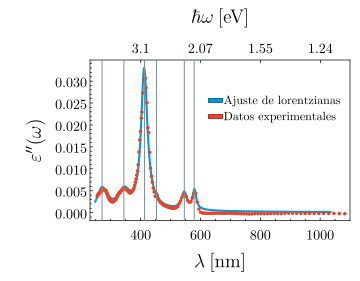
\includegraphics[width=0.47\textwidth]{../../Figuras/ajusteLorentz28.pdf}\label{subfig:ajusteLorentz15}}}\hspace{0.1cm}
	\sidesubfloat[Second image]{\hspace{-0.6cm}{		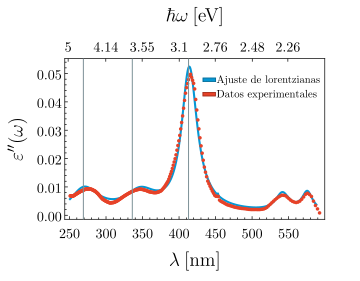
\includegraphics[width=0.46\textwidth]{../../Figuras/ajusteLorentz30.pdf}\label{subfig:ajusteLorentz28}}}\\
	\vspace{0.5cm}
	\sidesubfloat[Second image]{\hspace{-0.6cm}{		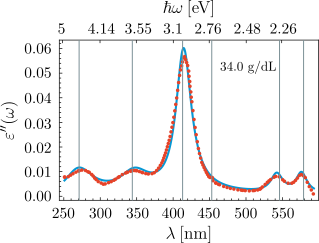
\includegraphics[width=0.47\textwidth]{../../Figuras/ajusteLorentz34.pdf}\label{subfig:ajusteLorentz30}}}\hspace{0.1cm}
	\sidesubfloat[Second image]{\hspace{-0.8cm}{		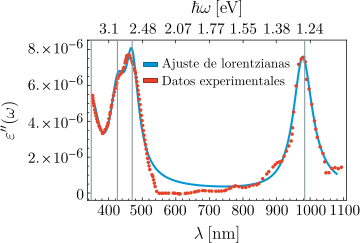
\includegraphics[width=0.52\textwidth]{../../Figuras/ajustePlasma.pdf}\label{subfig:ajusteLorentzPlasma}}}

	\caption{Parte imaginaria de la función dieléctrica como función de la longitud de onda $\lambda$ (eje inferior) y la energía $\hbar\omega$ (eje superior). Se grafican datos experimentales representados por puntos rojos y el ajuste con lorenzianas con una línea azul continua para \textbf{a)} eritrocitos con una concentración de 28.7 g/dL, cuyos experimentales se obtuvieron de \cite{friebelModelFunctionCalculate2006}; \textbf{b)} eritrocitos con una concentración de 230.6 g/dL, cuyos experimentales se obtuvieron de \cite{friebelDeterminationComplexRefractive2005a}; \textbf{c)} eritrocitos con una concentración de 34.0 g/dL, cuyos experimentales se obtuvieron de \cite{friebelDeterminationComplexRefractive2005a} y \textbf{d)} plasma, cuyos datos experimentales  se extrajeron de \cite{meinkeOpticalPropertiesPlatelets2007a}. En todas las figuras las líneas grises verticales indican las frecuencias de resonancia asociadas a los osciladores de Lorentz empleados en el ajuste.}
	\label{fig:epsLorentz}
\end{figure}
%

